\documentclass{homework}
\author{Zayn Wang, written in \LaTeX}
\title{Homework}

\graphicspath{{./media/}}

\begin{document} \maketitle

\newcommand\degree{^\circ}

\newcommand\rarr{\rightarrow}

\newcommand\rArr{\Rightarrow}

% \question xxx
% ans xxx

% 3.5 5.3

\question
% Vector?
$$ t_1 = 200m \div 5.0m/s = 40s, t_2 = 280m \div 4.0m/s = 70s, t = t_1 + t_2 = 110s
$$
$$ v_{avr} = \frac{d_1 + d_2}{t} = \frac{200m + 280m}{100s} = 4.3636m/s, \vec{v}_{avr} = \frac{\vec{d_1} + \vec{d_2}}{t} = \frac{200m - 280m}{110s} = -0.7273m/s
$$

\question

$$ \vec{v}_A = \vec{v}_B = \frac{40m - 20m}{3s - 0s} = 6.6667m/s, \vec{v}_c = 0, \vec{v}_D = \vec{v}_E = \vec{v}_F = \frac{0 - 40m}{6s - 5s} = -40m/s, \vec{v}_G = 0
$$

\question

$$(1)
$$
$$ \vec{v}(t) = \frac{dx}{dt} = (9.60m/s^2)t - (0.600m/s^6)t^5, \vec{v}(t_0) = (9.60m/s^2)t_0 - (0.600m/s^6)t_0^5 = 0 \rArr t_0 = 2s
$$
$$ \vec{x}_0 = 2.17m + (4.80m/s^2)(2s)^2 - (0.100m/s^6)(2s)^6 = 14.97m
$$
$$ \vec{a}(t) = \frac{dv}{dt} = 9.60m/s^2 - (3.000m/s^6)t^4, \vec{a}(t_0) = -38.4m/s^2
$$
$$(2)
$$
\begin{figure}[ht!]
    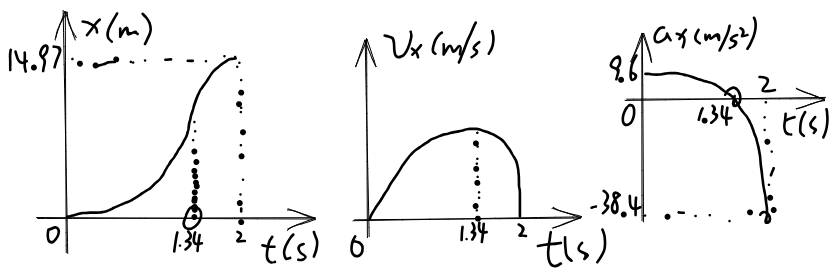
\includegraphics[width=12cm]{homework.png}
\end{figure}

\question

$$(a\&b)
$$
$$ \vec{v}(t) = \int{a(t)}dt = at + C, \because \vec{v}(0) = 0 \therefore \vec{v}(t) = at, at_f = 20m/s
$$
$$ \vec{x}(t) = \int{\vec{v}(t)}dt = \frac{1}{2}at^2 + C, \vec{x}(0) = 0, \vec{x}(t) = \frac{1}{2}at^2 \rArr \frac{1}{2}at_f^2 = 120m
$$
$$ a = 1.6667m/s^2, t_f = 12s
$$
$$(c)
$$
$$ d = 20m/s \times t_f = 240m
$$

\question

$$ The \ same \ as \ above: at_f = 3.8m/s, \frac{1}{2}at_f^2 = 6.80m \rArr a = 1.062m/s^2
$$
$$ \frac{1}{2}at_1^2 = 3.40m \rArr t_1 = 2.531s \rArr v(t_1) = at_1 = 2.687m/s
$$

\question

$$ Assume \ g = -10m/s^2
$$
$$(a)
$$
$$ t_h = \frac{0 - 20m/s}{-10m/s^2} = 2s, x = \frac{1}{2}gt^2 + v_0t + 50m = 70m
$$
$$(b)
$$
$$ from \ the \ highest \ point: v = gt, x = \frac{1}{2}gt^2 \rArr v^2 = 2gs \rArr v = -10\sqrt{14} m/s \approx -37.42m/s
$$
$$(c)
$$
$$ t = \frac{(-10\sqrt{14})m/s - 20m/s}{g} \approx 5.742s
$$

\question

$$ \Delta\vec{d} = (5.3m - 1.1m, -0.5m - 3.4m) = (4.2m, -3.9m)
$$
$$ \vec{v} = \frac{|\Delta\vec{d}|}{\Delta t} = 5.731m/s
$$
$$ Direction: \arctan(\frac{3.9}{4.2}) = 42.8789 \degree \ below \ the \ x-axis
$$

\question

$$ \vec{d} = d_0 + \vec{v} \cdot t = (-3.8m/s, 4.9m/s) \cdot 12s = (-45.6m, 58.8m), |\vec{d}| = 74.41m
$$

\question
$ \rArr 9t^2 + 2
$

\question
% Unit?
$$ v(t) = \frac{dr}{dt} = 3t^2 - 4 = 0 \rArr t = \sqrt{\frac{4}{3}}s \therefore r(t) = 10 - \frac{8}{3}\sqrt{\frac{4}{3}} m
$$

\end{document}